%23.10.2024, lecture 3

\section{Coding}

\begin{definition}
    Let $\mathcal{A} = \{ a_{1}, a_{2}, \dots, a_{n} \}$ be an alphabet.
    A \emph{code} is a function $C: \mathcal{A} \to \{ 0, 1 \}^{\ast}$ which assigns codewords to the letters of the alphabet.
    If every message obtained by applying the code $C$ can be decoded uniquely, then the code is called uniquely decodable.
\end{definition}

We say that $c$ is a \emph{codeword} of the code $C$ if $c = C(a)$ for some $a \in \mathcal{A}$.

\begin{theorem} [Kraft-McMillan Inequality]
    \label{thm:Kraft-McMillan}
    For every uniquely decodable code with codewords $\{ c_{1}, c_{2}, \dots, c_{n} \}$, the following holds:
    \[
        \sum _{ i = 1 }^{ n } 2^{-|c_{i}|} \le 1.
    \]
\end{theorem}

\begin{proof}
    Idea.
    Let $p_{i}$ be a probability of $a_{i}$, where $p_{i} \approx 2^{-|c_{i}|} \implies |c_{i}| \approx - \log p_{i}$

    Let $\{ c_{1}, c_{2}, \dots, c_{n} \}$ be uniquely decodable

    \[
        \sum _{ i = 1 }^{ n } 2^{-|c_{i}|} \le 1
    \]

    Let's define a monomial for each code (assume that our ring is not commutative):
    If $c_{i} = 0101101$, then $p_{i}(x, y) = xyxyyxy$ and so on.
    Now, let's define a polynomial (for now, assume that $L$ is just some number):
    \begin{align*}
        f(x, y) &= \left( \sum _{ i = 1 }^{ n }  p_{i}(x, y) \right)^{L}  \\
        &= \sum _{ l = L }^{ L \cdot \max |c_{i}| } M_{l}(x, y)\text{, where } M_{l}(x, y) \text{is a sum of all monomials of degree } l.
    \end{align*}

    As codes are uniquely decodable, one can say that every monomial occurs in $M_{l}$ at most once.
    Hence $\# \{ \text{monomials of degree } l \} \le 2^{l}$.
    Thus we have:
    \[
        f\left( \frac{1}{2}, \frac{1}{2} \right) \leq \sum _{ l = L }^{ L \cdot \max |c_{i}| } 2^{l} \cdot \left( \frac{1}{2} \right)^{l} \le L \cdot \max |c_{i}| = O(L).
    \]
    Now, assume that $\sum_1^n 2^{-|c_{i}|} > 1 \implies \sum_1^n {2}^{-|c_{i}|}  = 1 + \varepsilon$ for some $\varepsilon > 0$.
    Note several facts:
    \begin{enumerate}
        \item $f\left( \frac{1}{2}, \frac{1}{2} \right) = O(L)$.
        \item $f\left( \frac{1}{2}, \frac{1}{2} \right) = \left( \sum_{i = 1}^n 2^{-|c_{i}|} \right)^{L} = (1 + \varepsilon)^{L}$ (since $p_{i}\left( \frac{1}{2}, \frac{1}{2} \right) = 2^{-|c_{i}|}$).
    \end{enumerate}
    Hence, we have a contradiction.
\end{proof}

\subsection{Prefix-Free Codes}

\begin{definition}
    A code is called prefix (prefix-free) if no codewords is a prefix of another codeword.
\end{definition}


\begin{theorem} [Kraft-McMillan Inequality for prefix codes]
    For prefix code with codewords $\{ c_{1}, c_{2}, \dots, c_{n} \}$:
    \[\sum_{i = 1}^{n}2^{-l_{i}} \le 1,\]
    where $l_i = |c_i|$.
\end{theorem}
\begin{proof}
    For each node in the tree at depth $k$ one can assign a probability $\frac{1}{2^{k}}$.
    Hence, for a leaf $c_i$ we will have the probability $2^{-l_i}$, but the sum over all leaves is 1.
    See~\Cref{fig:image_2024-10-23_22-13-28}.
    \begin{figure}[H]
        \centering
        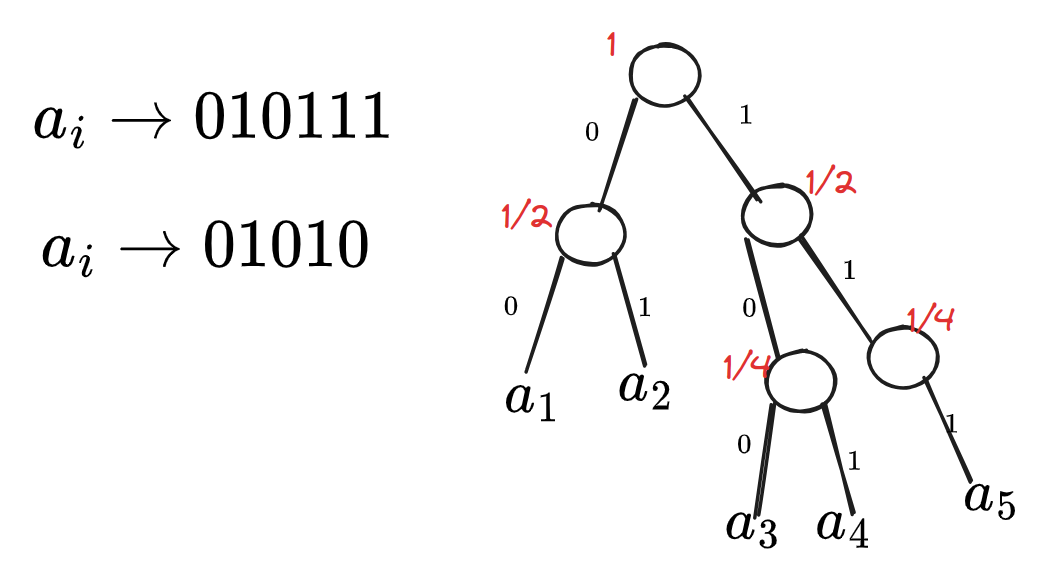
\includegraphics[width=0.5\textwidth]{figures/image_2024-10-23_22-13-28}
        \caption{Probabilities on a prefix code.}
        \label{fig:image_2024-10-23_22-13-28}
    \end{figure}
\end{proof}

The reverse statement is also correct:
\begin{theorem}
    For a set of integers $\{ l_{1}, l_{2}, \dots, l_{n} \}$ that satisfies $\sum _{ i = 1 }^{ n } 2^{-l_{i}} \le 1$, there exists a prefix code with codewords $\{ c_{1}, c_{2}, \dots, c_{n} \}$ where $|c_{i}| = l_{i}$.
\end{theorem}
\begin{proof}
    At first, we create a binary tree with leaves at depths: $\{ l_{1}, l_{2}, \dots, l_{n} \}$ .
    Each leaf will be a codeword.

    Take a segment $[0, 1]$ and place each $2^{-l_i}$ on it in the desceding order.
    Start taking its parts greedily
    Then, you can construct . \todo{todo}
    $\text{Segment} \longleftrightarrow \text{Tree} \longleftrightarrow \text{codewords with} \sum _{ i = 1 }^{ n } 2^{-l_i} \le 1$
\end{proof}

\begin{corollary}
    For any unique decodable code, there exists a prefix code with the same length of codewords.
\end{corollary}

\subsubsection{Lower Bound}

\begin{theorem}[Shanon]
    For any distribution of letters $\alpha$ and any uniquely decodable code (so probability of symbol $a_i$ is $p_i$ and its code is $c_i$), the following holds:
    \[
        \text{Average code length} =  \sum _{ i = 1 }^{ n } p_{i} \cdot |c_{i}| \ge \sum _{ i = 1 }^{ n } p_{i} \cdot \log \frac{1}{p_{i}} = H(\alpha).
    \]
\end{theorem}

Since we have distribution $\alpha$, then we need at least $H(\alpha)$ bits to encode a symbol. \todo{not sure what i've just said}
\begin{proof}
    Move everything to the right side and apply Jensen's inequality:
    \begin{align*}
        \sum _{ i = 1 }^{ n } p_{i} \cdot \log \frac{2^{-|c_{i}|}}{p_{i}}
        &\le \log \sum _{ i = 1 }^{ n } \left( p_{i} \frac{2^{-|c_{i}|}}{p_{i}} \right)  \\
        &= \log \sum _{ i = 1 }^{ n } 2^{-|c_{i}|} \\
        &\le \log 1 = 0. \\
    \end{align*}
\end{proof}

\subsubsection{Upper Bound}

\begin{theorem}[Shannon]
    For every distribution $\alpha = \{ p_{1}, p_{2}, \dots, p_{n} \}$ there exists a prefix code $\{ c_{1}, c_{2}, \dots, c_{n} \}$:
    \[
        \sum _{ i = 1 }^{ n } p_{i} \cdot |c_{i}| \le \left(\sum _{ i = 1 }^{ n } p_{i} \cdot \log \frac{1}{p_{i}}\right) + 1 = H(\alpha) + 1.
    \]
\end{theorem}
\begin{proof}
    Let $l_{i} = \left\lceil  \log \frac{1}{p_{i}}  \right\rceil$.
    Note that $\{ l_{i} \}$ satisfy the Kraft-McMillan inequality~\ref{thm:Kraft-McMillan}:
    \begin{align*}
        \sum _{ i = 1 }^{ n } 2^{-|c_{i}|} &= \sum _{ i = 1 }^{ n } 2^{-\lceil \log 1/p_{i} \rceil }  \\
        &\le \sum _{ i = 1 }^{ n } 2^{-\log 1/p_{i}} \\
        &= \sum_{i =1}^{n} p_{i} \\
        &= 1.
    \end{align*}
    Let's estimate the average code length:
    \begin{align*}
        \sum _{ i = 1 }^{ n } p_{i} \cdot l_i &= \sum _{ i = 1 }^{ n } p_{i} \cdot \left\lceil  \log \frac{1}{p_{i}}  \right\rceil  \\
        &< \sum _{ i = 1 }^{ n } p_{i} \cdot \left( \log \frac{1}{p_{i}} + 1 \right) \\
        &= \left( \sum_{i = 1}^{n}p_{i} \cdot \log \frac{1}{p_{i}} \right) + 1.
    \end{align*}
\end{proof}

\subsubsection{Examples}

\begin{example}[Shannon-Fano Code]
    Assume that $p_{1} \ge p_{2} \ge \dots \ge p_{n}$, and assign it to the sub-segments of $[0, 1]$.
    All codes in $\left[ 0, \frac{1}{2} \right]$ starts with $0$, all others start with $1$. Continue recursively.
    \begin{figure}[H]
        \centering
        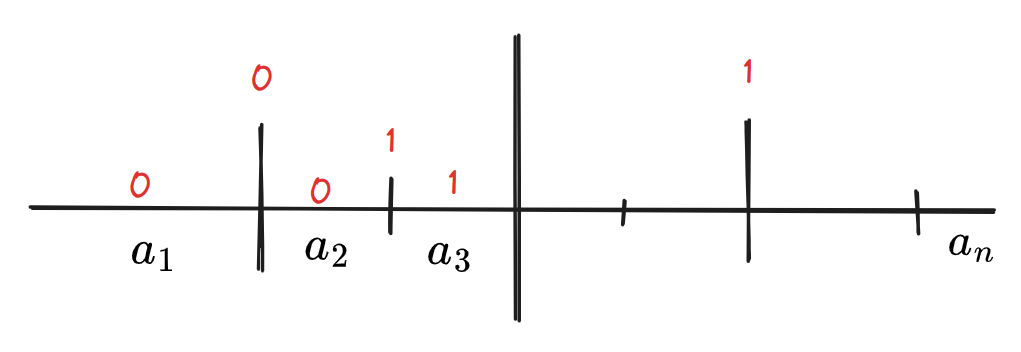
\includegraphics[width=0.5\textwidth]{figures/telegram-cloud-document-2-5244613392966114247}
        \caption{Shannon-Fano code.}
        \label{fig:telegram-cloud-document-2-5244613392966114247}
    \end{figure}
    Obviously, it is a prefix-free code
    See \Cref{fig:telegram-cloud-document-2-5244613392966114247}.
\end{example}

\begin{example}[Huffman Code]
	We're given with probabilities $p_1, \ldots, p_n$.
	Let's create a binary tree with weights in nodes.
	Initially, we have $n$ leaves and each leaf has weight $p_i$.
	On each step, take two roots of different components with the smallest weights and merge them into one node with the weight equal to the sum of the weights of the two nodes.
	At the end, you will have a binary tree with $p_i$ in the leaves.
	Now, assign $0$ to the left edge and $1$ to the right edge.
	Then, path to each leaf will be a code for the corresponding letter.

    \todo[inline]{complete haffman code}
    Huffman is an optimal code.
    To prove that, one needs both Shannon theorems.
    Assume that $p_{1} \ge p_{2} \ge \dots \ge p_{n}$.
    Use greedy algorithm to build a Huffman Tree.
\end{example}

\subsubsection{Summary}

\begin{itemize}
    \item For every uniquely decodable code there is a prefix code with the same code length.
    \item The average code length of the optimal code is related to Shannon Entropy:
    \[
        H(\alpha) \le \sum _{ i = 1 }^{ n } p_{i} \cdot |c_{i}| \le H(\alpha) + 1.
    \]
    \item The $+1$ on the right side cannot be eliminated: for example, if we have only two symbols in the alphabet, then $\sum p_{i} \cdot |c_{i}| = 1$, while $\sum p_{i} \cdot \log \frac{1}{p_{i}}$ can be arbitrarily close to zero.
    For example, for any $\eps > 0$ there is a code with probabilities:

    \begin{center}
    \begin{tabular}{|c|c|c|}
        \hline
        $a_{i}$ & $p_{i}$ & $|c_{i}|$ \\
        \hline
        $a_{1}$ & $\varepsilon$ & 1 \\
        $a_{2}$ & $1 - \varepsilon$ & 1 \\
        \hline
    \end{tabular}
    \end{center}
\end{itemize}

\subsection{Block Coding}

Now we encode not individual symbols but blocks of symbols.
Let each block consist of $k$ symbols.
Let the random variables $\alpha_{1}, \alpha_{2}, \dots, \alpha_{k}$ be distributed as $\alpha$ and correspond to the letters in the block.
\[
H(\alpha_{1}, \alpha_{2}, \dots, \alpha_{k}) = \sum_{i = 1}^{k} H(\alpha_{i}) = k \cdot H(\alpha)
\]
Due to Shannon's theorems, we have the following:
\[
H(\alpha) \le \text{[average length of the letter code in the block]} \le H(\alpha) + \frac{1}{k}.
\]

Note that when coding blocks of length 100, we achieved a deviation from entropy of no more that $0.01$. However, we cannot apply the Huffman code since the algorithm for its construction \todo{finish}

\subsubsection{Arithmetic Coding}

\todo[inline]{no idea}

\begin{definition}
    Assume that $p_{1} \ge p_{2} \ge \dots \ge p_{n}$ and assign it to the subsegements of $[0, 1]$ (all numbers below are base 2 and we omit $0.$ at their beginning, since all of them in $[0, 1)$).
    We say that half-open interval is \emph{standard} if it has the form $[v 0, v 1]$, where $v \in \{ 0, 1 \}^{\ast}$.
    We will assign to each standard interval $[v 0, v1]$ the code $v0$ю
\end{definition}

\begin{statement}
    Arithmetic coding is not as optimal.
\end{statement}
\begin{proof}
    \[\sum _{ i = 1 }^{ n } p_{i} \cdot |c_{i}| \le \sum _{ i = 1 }^{ n } p_{i} \cdot \log \frac{1}{p_{i}} + 2. \qedhere \]
\end{proof}

\subsubsection{Block Coding With Errors}

Let $\alpha_{1}, \alpha_{2}, \dots, \alpha_{n}$ be i.i.d. random variables on $\{ a_{1}, a_{2}, \dots, a_{k} \}$ with probabilities $p_{1}, p_{2}, \dots, p_{k}$.
Consider block coding defined by functions $E_{n}$ and $D_{n}$:
\begin{itemize}
    \item $E_{n}: \{ a_{1}, a_{2}, \dots, a_{k} \}^{n} \to \{ 0, 1 \}^{L_{n}}$.
    \item $D_{n}: \{ 0, 1 \}^{L_{n}} \to \{ a_{1}, \dots, a_{k} \}^{n}$.
\end{itemize}

The error probability $\varepsilon_{n}$ is the probability of the following event:
\[
\left[ (\alpha_{1}, \alpha_{2}, \dots, \alpha_{n}) = (a_{i_{1}}, a_{i_{2}}, \dots, a_{i_{n}}) \mid D_{n}(E_{n}(a_{i_{1}}a_{i_{2}}, \dots, a_{i_{n}})) \ne (a_{i_{1}}, a_{i_{2}}, \dots, a_{i_{n}}) \right].
\]


